All those sequencing techniques are aimed to investigate only one cellular compartment at a time, but in order to obtain a more comprehensive view of the cellular behaviour, it is necessary to look at more than one -omic at the same time.

\begin{figure}[h]
\centering
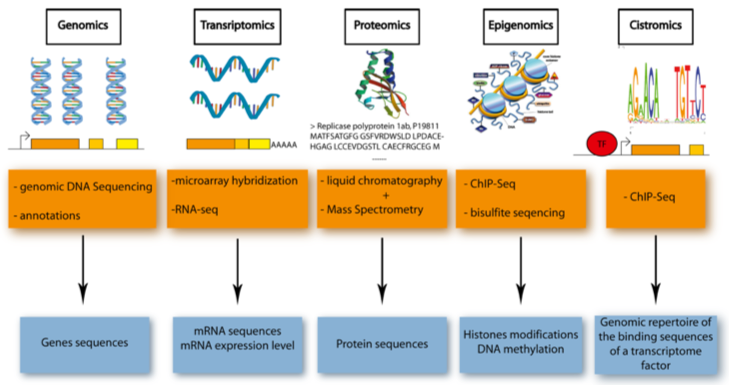
\includegraphics[width=8cm, keepaspectratio]{img/intro/omics.png}
\caption[Omics Representation]{}
\label{fig:omics}
\end{figure}

Indeed, we can imagine each omic as a camera in a multi-view camera system pointed on a building from different point of view.
Each device takes snapshots of the building from different angles, but the information is still fragmented.
In order to reconstruct a 3D model of the building, we need to put the snapshots took from each device together.

\begin{figure}[h]
\centering
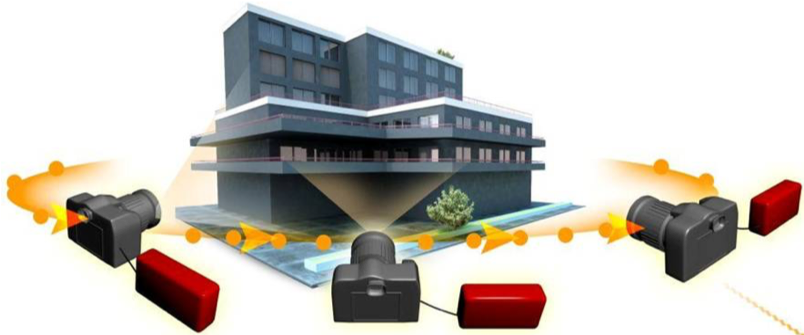
\includegraphics[width=8cm, keepaspectratio]{img/intro/cameras.png}
\caption[Integration cameras]{}
\label{fig:cameras}
\end{figure}

The same idea can be adapted to the sequencing techniques, we need to integrate information coming from different omics in order reconstruct (and understand) how multiple mechanisms orchestrate the cellular behavior.
As figure \ref{fig:funnell} outline, multi-omics data integration can be made at different levels, by graphical exploration, by functional annotation, by network fusion and by dimensionality reduction.

\begin{figure}[h]
\centering
\includegraphics[width=8cm, keepaspectratio]{img/intro/funnell.pdf}
\caption[Integration Funnell]{A schematic representation of multi-omic data integration levels.}
\label{fig:funnell}
\end{figure}

With graphical exploration, we can visualize data coming from different sources (e.g. \textit{RNA-seq} and \textit{ChIP-seq}) using specific tools designed at this scope, such as \textit{Genome Browser} \cite{Karolchik2011} or \gls{igv} \cite{Robinson2011, Thorvaldsdottir2013} and looking to the overlapping regions, or where expressed epigenomic markers have corrispondence with gene expression sites.

We refer to functional annotation integration when using methods combining analysis results (such as relevant lists of genes) with public available databases,  like the Gene Ontology\footnote{http://www.geneontology.org/} and pathway (\textit{KEGG}\footnote{https://www.genome.jp/kegg/} or \textit{Reactome}\footnote{https://reactome.org/}) based ones, to detect functional responses highly related to the experimental condition under investigation.

It is possible to integrate multiple omics data types by constructing multiple networks, one for each omic analyzed, and then combine these networks with fusion techniques.
This integration aspect is used when high number of data samples is available or when having multiple-omics data types coming from the same patients \cite{Wang2014}.

A deeper level of integration is achievable with dimensionality reduction techniques. 
Also in this case, several samples are needed to be able to obtain relevant and reliable results.
Generally speaking, these methods are able to start from multiple samples coming from different omics and to reduce their dimensionality, enabling to identify common cellular behavioral aspects \cite{Rohart2017,Argelaguet2018}.



